\section{Evaluation}
\begin{frame}[t]{Evaluation}
	\begin{itemize}
		\item Evaluation involves:
		      \begin{itemize}
			      \item Running the \emph{Jayvee} interpreter under specific configurations,
			      \item Compare the runtime
			      \item Compare the output tables
		      \end{itemize}
		\item Requires a dataset as input, with these requirements
		      \begin{description}
			      \item[CSV format] The interpreter can only transform CSV into tables
			      \item[openness] Licensed with an Open Definition\footnotemark[1] compliant licenses\footnotemark[2]
		      \end{description}
		\item Dataset is "Brewery Operations and Marked analysis"\footnotemark[3]
		      \begin{itemize}
			      \item No real-world data
		      \end{itemize}
	\end{itemize}
	\footnotetext[1]{\textcite{opendefinition}}
	\footnotetext[2]{\textcite{opendefinition:licenses}}
	\footnotetext[2]{\textcite{dataset}}
\end{frame}
\begin{frame}[t]{Evaluation}{Configurations}
	These characteristics define a configuration:\\
	\begin{tabular}{|l|l|}
		\hline
		characteristic   & possible values                                \\
		\hline
		backend          & TS, PL, PLOB, PLRS, PLOBRS                     \\
		transform amount & none (0), some (4), many (8)                   \\
		input rows       & 56250, 112500, 225000, 450000, 900000, 1800000 \\
		\hline
	\end{tabular}
	\only<2> {
		\begin{figure}
			\begin{subfigure}{0.2\linewidth}
				\centering
				\includesvg{assets/ts_cfg.ad.svg}
				\caption{TS, PL, PLRS}
			\end{subfigure}
			\begin{subfigure}{0.2\linewidth}
				\centering
				\includesvg{assets/plob_cfg.ad.svg}
				\caption{PLOB, PLOBRS}
			\end{subfigure}
			\caption{How configurations load the table}
		\end{figure}
	}
	\only<3>{
		\begin{figure}
			\begin{subfigure}{0.3\linewidth}
				\centering
				\includesvg{assets/no_cfg.ad.svg}
				\caption{none}
			\end{subfigure}
			% \hfill
			\begin{subfigure}{0.3\linewidth}
				\centering
				\includesvg[height=0.55\FrameHeight]{assets/so_cfg.ad.svg}
				\caption{some}
			\end{subfigure}
			% \hfill
			\begin{subfigure}{0.3\linewidth}
				\centering
				\includesvg[height=0.55\FrameHeight]{assets/ma_cfg.ad.svg}
				\caption{many}
			\end{subfigure}
			\caption{How configurations transform the table}
		\end{figure}
	}
\end{frame}

\begin{frame}
	\centering
	\large
	DEMO TIME!! % FIXME REWORD
\end{frame}

\begin{frame}[t]{Evaluation}{Maximum input size}
	\begin{itemize}
		\item The interpreter has a maximum size for all configurations, except with the PLOBRS backend
		\item There are three different types of errors:
		      \begin{enumerate}
			      \item "Invalid string lenght": likely a \emph{NodeJs} limitation on the maximum length of a string. It occurs when generating SQL insert statements for a table.
			      \item "JavaScript heap overflow": Also occurs when generating SQL insert queries.
			      \item "Cannot make a string longer than 0x1fffffe8 characters": Occurs when attempting to transform the binary file data into a string
		      \end{enumerate}
		      Crashes 1 and 2 are don't appear when using \Verb|sqlite-loader-lib|, crash 3 disappears when using a \Verb|LocalFileToTextInterpreter| block
	\end{itemize}
	\begin{figure}
		\centering
		\begin{tikzpicture}
			\scriptsize
			\begin{axis}[
					height = 0.37\textheight,
					xlabel = {transform amount},
					ylabel = {rows},
					xtick = {1,2,3},
					xticklabels={none,some,many},
					legend pos=south west,
				]
				\addplot[
					color = red,
					mark=triangle*,
				]
				coordinates {
						(1,1900000)(2,1300000)(3,900000)
					};
				\addlegendentry{TS}
				\addplot[
					color=blue,
					mark=triangle*,
				]
				coordinates {
						(1,1800000)(2,1800000)(3,1700000)
					};
				\addlegendentry{PL}
				\addplot[
					color=brown,
					mark=triangle*,
				]
				coordinates {
						(1,1900000)(2,1700000)(3,1700000)
					};
				\addlegendentry{PLOB}
				\addplot[
					color=green,
					mark=triangle*,
				]
				coordinates {
						(1,2000000)(2,2000000)(3,2000000)
					};
				\addlegendentry{PLRS}
			\end{axis}
		\end{tikzpicture}
	\end{figure}
\end{frame}

\begin{frame}[t]{Evaluation}{Execution Duration}
	\begin{columns}[T]
		\begin{column}{0.5\linewidth}
			\begin{description}
				\item[PL] Slower than TS for no and some transforms.
				      However, PL is faster with many transforms.
				      This suggests, that PL's transform implementation is superior.

				\item[PLOB] Faster than TS.
				      This suggests, that PLOB's table parsing implementation is superior.

				\item[PLRS] Faster than TS.
				      This suggests, that \Verb|sqlite-loader-lib|'s table export implementation is superior.

				\item[PLOBRS] Fastest. Combines the advantages of PL, PLOB and PLRS
			\end{description}
		\end{column}
		\begin{column}{0.5\linewidth}
			\tiny
			\begin{figure}
				\centering
				\begin{tikzpicture}
					\begin{axis}[
							height = 0.25\textheight,
							width = 0.8\textwidth,
							% xlabel = {rows},
							ylabel = {time in ms},
							ymin=0, ymax=150000,
							xmin=0, xmax=1800000,
							legend pos=north west,
						]
						\addplot[
							color = red,
							mark=triangle*,
						]
						coordinates {
								(56250,3724)(112500,6648)(225000,12202)(450000,25701)(900000,47064)(1300000,68801)(1800000,96513)
							};
						\addplot[
							color=blue,
							mark=triangle*,
						]
						coordinates {
								(56250,4581)(112500,8323)(225000,16118)(450000,34125)(900000,63728)(1300000,93559)(1800000,139939)
							};
						\addplot[
							color=brown,
							mark=triangle*,
						]
						coordinates {
								(56250,2531)(112500,4231)(225000,7739)(450000,14976)(900000,30211)(1300000,42888)(1800000,64660)
							};
						\addplot[
							color=green,
							mark=triangle*,
						]
						coordinates {
								(56250,3102)(112500,5390)(225000,10126)(450000,21270)(900000,37705)(1300000,54562)(1800000,74755)
							};
						\addplot[
							mark=triangle*,
						]
						coordinates {
								(56250,1035)(112500,1221)(225000,1936)(450000,2740)(900000,4526)(1300000,6060)(1800000,8184)
								%PL slopes: 0,003306667+0,006355556+0,003573333+0,003968889+0,003068+0,004248: 0,004086741
							};

						\legend{TS,PL,PLOB,PLRS,PLOBRS}
					\end{axis}
				\end{tikzpicture}
				\begin{tikzpicture}
					\begin{axis}[
							height = 0.25\textheight,
							width = 0.8\textwidth,
							% xlabel = {rows},
							ylabel = {time in ms},
							xmin=0, xmax=1800000,
							ymin=0, ymax=150000,
							legend pos=north east,
						]
						\addplot[
							color = red,
							mark=*,
						]
						coordinates {
								(56250,4495)(112500,8283)(225000,15346)(450000,32467)(900000,60755)(1300000,95102)
							};
						\addplot[
							color=blue,
							mark=*,
						]
						coordinates {
								(56250,4825)(112500,8952)(225000,16881)(450000,36874)(900000,67674)(1300000,99959)
							};
						\addplot[
							color=brown,
							mark=*,
						]
						coordinates {
								(56250,2804)(112500,4756)(225000,8544)(450000,16524)(900000,33375)(1300000,49007)
							};
						\addplot[
							color=green,
							mark=*,
						]
						coordinates {
								(56250,3144)(112500,5479)(225000,9894)(450000,21076)(900000,37910)(1300000,57910)
							};
						\addplot[
							mark=*,
						]
						coordinates {
								(56250,1106)(112500,1305)(225000,1789)(450000,2396)(900000,4323)(1300000,6252)
							};

						\legend{TS,PL,PLOB,PLRS,PLOBRS}
					\end{axis}
				\end{tikzpicture}
				\begin{tikzpicture}
					\begin{axis}[
							height = 0.25\textheight,
							width = 0.8\textwidth,
							xlabel = {rows},
							ylabel = {time in ms},
							xmin=0, xmax=1800000,
							ymin=0, ymax=150000,
							legend pos=north east,
						]
						\addplot[
							color = red,
							mark=square*,
						]
						coordinates {
								(56250,5722)(112500,11097)(225000,18750)(450000,38264)(900000,81900)
							};
						\addplot[
							color=blue,
							mark=square*,
						]
						coordinates {

								(56250,5421)(112500,10348)(225000,17914)(450000,35151)(900000,72515)

							};
						\addplot[
							color=brown,
							mark=square*,
						]
						coordinates {

								(56250,3064)(112500,5248)(225000,9470)(450000,18147)(900000,35656)

							};
						\addplot[
							color=green,
							mark=square*,
						]
						coordinates {
								(56250,3545)(112500,5997)(225000,10051)(450000,24406)(900000,38963)
							};
						\addplot[
							mark=square*,
						]
						coordinates {
								(56250,1178)(112500,1383)(225000,1668)(450000,2627)(900000,4518)
							};

						\legend{TS,PL,PLOB,PLRS,PLOBRS}
					\end{axis}
				\end{tikzpicture}
			\end{figure}
		\end{column}
	\end{columns}
\end{frame}

\begin{frame}[t]{Evaluation}{TS compared to PLOBRS}
	\begin{columns}[T]
		\begin{column}{0.5\linewidth}
			\begin{itemize}
				\item The three curves are monotonously rising \\
				      \textrightarrow
				      \text{} As the number of rows increases, the PLOBRS backend's processing speed compared to TS increases
				\item The curve representing a pipeline with many transforms, lies above the curve representing some transforms, which itself lies above the curve representing no transforms \\
				      \textrightarrow
				      \text{} The greater the number of transforms in a pipeline, the faster the PLOBRS backend is in comparison to the TS baseline
			\end{itemize}
		\end{column}
		\begin{column}{0.5\linewidth}
			\begin{figure}
				\centering
				\begin{tikzpicture}
					\begin{axis}[
							height=0.7\textheight,
							width=0.8\textwidth,
							xlabel = {rows},
							ylabel = {TS / PLOBRS},
							xmin=0, xmax=1800000,
							legend pos=south east,
						]
						\addplot[
							color = red,
							mark=triangle*,
						]
						coordinates {
								(56250,3.60)(112500,5.31)(225000,6.22)(450000,9.34)(900000,10.40)(1300000,11.35)(1800000,11.80)
							};
						\addlegendentry{none}
						\addplot[
							color = blue,
							mark=*,
						]
						coordinates {
								(56250,4.06)(112500,6.35)(225000,8.58)(450000,13.55)(900000,14.06)(1300000,15.22)
							};
						\addlegendentry{some}
						\addplot[
							mark=square*,
						]
						coordinates {
								(56250,4.86)(112500,8.02)(225000,11.24)(450000,14.57)(900000,18.22)
							};
						\addlegendentry{many}
					\end{axis}
				\end{tikzpicture}
			\end{figure}
		\end{column}
	\end{columns}
\end{frame}
\begin{frame}[t]{Evaluation}{Differences in resulting tables}
	\begin{itemize}
		\item Differing floating point values
		      \begin{itemize}
			      \item Transforms that work with floating point values produce differing outputs
			      \item Seemingly random
			      \item About every 1074 rows
			      \item $\num{8.53e-9}$ average difference
			      \item Probably caused by an implementation difference between \emph{TypeScript} and \emph{Polars}
		      \end{itemize}
		\item Rows including \Verb|NULL|
		      \begin{itemize}
			      \item Original implementation: Replace with empty string or discard row
			      \item New implementation: Has rows with \Verb|NULL|
		      \end{itemize}
	\end{itemize}

\end{frame}

\begin{frame}[t]{Evaluation}{Functional requirements}
	\begin{description}
		\item[columnar] A columnar format has advantages described previously, including faster read times and less memory usage \uncover<2->{({\color{green} \checkmark})}
		\item[interoperability] This allows the data to be used by multiple different applications without complex conversion \uncover<3->{({\color{green} \checkmark})}
		\item[feature toggle] We must be able to (de)activate the new features at runtime \uncover<4->{({\color{green} \checkmark})}
		\item[compatibility] The \Verb|.sqlite| files produced by the different implementations must be identical \uncover<5->{({\color{red} \xmark})}
		\item[modularization] Should it be necessary to write code in a language other than \emph{TypeScript}, this code must be placed in an external library usable from \emph{TypeScript} \uncover<6->{({\color{green} \checkmark})}
		\item[extensibility] The functionality of the chosen data representation must be extensible \uncover<7->{({\color{green} \checkmark})}
	\end{description}
\end{frame}

\begin{frame}[t]{Evaluation}{Non-functional Requirements}
	\begin{description}
		\item[performance] Either a decrease in the execution time for \emph{Jayvee} models, or an extension of the \emph{Jayvee} interpreter's capabilities \uncover<2->{({\color{green} \checkmark})}
		\item[code style] The source code adheres to the project's code style \uncover<3->{({\color{green} \checkmark})}
		\item[maturity] We aim to create a prototype, not a mature implementation \uncover<4->{({\color{green} \checkmark})}
	\end{description}
\end{frame}

